%----------------------------------------------------------------------------
\chapter{Experiments and results}\label{sect:Experiments}
%----------------------------------------------------------------------------
\section{Evaluation methods}

I used three methods to evaluate the results. The most basic method is the accuracy measure, which calculates the ratio of the correct answers as follows:

\[accuracy = \frac{correct\ answer}{all\ answer}\]

Since we are talking about graphs we need to measure the accuracy on the nodes and (if we are also training on them) the edges.
\[accuracy_{nodes\ and\ edges} = \frac{correct\ nodes + correct\ edges}{all\ nodes + all\ edges}\]

The other general evaluation metric in case of classification is the F-score. This is better for evaluating the results of a classification because it is not so greatly affected by the distribution of the classes. For this we need to calculate the true positive, true negative, false positive and false negative measures for every class. See on Figue~\ref{fig:TP_TN_FP_FN}.

\begin{figure}[!ht]
	\centering
	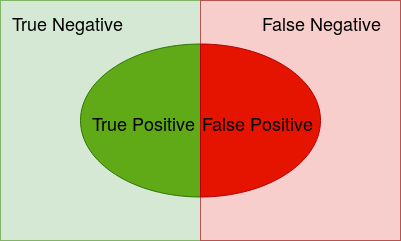
\includegraphics[width=100mm, keepaspectratio]{figures/F_score.png}
	\caption{The visual representation of the concept of true positive, true negative, false positive and false negative measures.}
	\label{fig:TP_TN_FP_FN}
\end{figure}


\[TP_{node==0} = number\ of\ correctly\ guessed\ node==0\]
\[TN_{node==0} = number\ of\ correctly\ guessed\ node!=0\]
\[FP_{node==0} = number\ of\ incorrectly\ guessed\ node==0\]
\[FN_{node==0} = number\ of\ incorrectly\ guessed\ node!=0\]

With these measures we can calculate the precision and recall. The precision tells us the ratio of correct guesses of the class out of every time the model predicted that class. The recall is the ratio of the correct guesses out of every instance that are actually in the class. The harmonic mean of the precision and recall is the F-score.

\[precision = \frac{TP}{TP + FN}\]
\[recall = \frac{TP}{TP + FP}\]

\[F1 = 2 * \frac{precision * recall}{precision + recall}\]

I constructed extractive summaries from the resulting graphs and the original articles multiple ways described in section~\ref{ssect:ExperimnetsAndResults} and calculated the various ROUGE scores for each method's output.

\section{Experiments and results}\label{ssect:ExperimnetsAndResults}
I have experimented with both the Encode Process Decode and the Graph Attention Network models with varying success.
\subsection{Encode Process Decode}
At first I tried to get the Encode-Process-Decode model to predict whether to put something in the summary graph or not using only the word ids as features, but realized it would probably be more sufficient to also use the POS tags.

I also experimented with different loss functions, but for now i decided to use softmax cross entropy with output feature sizes of 2. This loss function is also available in the Appendices\ref{sect:Appendices}.

Training on more, than 7000 article for 5 epochs (Early stopping stopped it from running any longer) I've got the following results.
\begin{table}[!h]
	\centering
	\begin{tabular}{| c | c |}
		\hline
		Test loss & 0.447 \\ \hline
		Correct test parts & 0.958 \\ \hline
		Correctly solved test graphs & 0.0 \\ \hline
	\end{tabular}
	\caption{Softmax cross entropy loss and accuracy on the test set}
\end{table}

\begin{table}[!h]
	\centering
	\begin{tabular}{| c | c | c | c |}
		\hline
		 & precision & recall & f1 \\ \hline \hline
		edges0&0.96&1.0&0.98  \\ \hline
		edges1 & 0.0 & 0.0 & 0.0 \\ \hline
		nodes0 & 0.915 & 0.985 & 0.949 \\ \hline
		nodes1 & 0.628 & 0.213 & 0.319 \\ \hline
	\end{tabular}
	\caption{The classification report on the test set}
\end{table}

As it is clear from this the network hardly ever classifies a node as "1", meaning that is should be in the summary graph, but when it does it is 62.8\% accurate.

This model has not been further evaluated.

\subsection{SimpleGraphAttention Network}
I trained the network on the whole training set (80\% of the whole dataset) for 3 epochs. It stopped after the third epoch because of the early stopping mechanism.

I evaluated the trained network on the test set and the results are the following:

\begin{table}[!h]
	\centering
	\begin{tabular}{| c | c |}
		\hline
		Test loss & 0.809 \\ \hline
		Correct test parts & 0.724 \\ \hline
		Correctly solved test graphs & 0.0 \\ \hline
	\end{tabular}
	\caption{Softmax cross entropy loss and accuracy on the test set}
\end{table}

\begin{table}[!h]
	\centering
	\begin{tabular}{| c | c | c | c |}
		\hline
		& precision & recall & f1 \\ \hline \hline
		nodes0 & 0.819 & 0.814 & 0.816 \\ \hline
		nodes1 & 0.534 & 0.542 & 0.538 \\ \hline
	\end{tabular}
	\caption{The classification report on the test set}
\end{table}

\subsubsection{Summary reconstruction and evaluation}
I tried three different approaches at the summary extraction, each have been evaluated by the ROUGE scoring mechanism. For this I used the perl based pyrouge package.

\paragraph{Reconstruction with the node average}

This reconstruction method scores each sentence of the original article using the equation below where the \(score_{word}\) is the predicted probability of the word (node) being in the summary graph.

\[score_{sentence} = \frac{\sum_{word \in sentence\ and\ word \notin stopwords} score_{word}}{|word \in sentence\ and\ word \notin stopwords|}\]

Based on the calculated score of each sentence we can order them by their relevance and keep the four most relevant sentence from the article as the summary.

This method does not utilize the information of the graph structure nor does it prefer longer sentences.

\begin{longtable}{| l | l | l |}
	\hline
	\textbf{Evaluation method}&\textbf{Metric}&\textbf{Score}\\ \hline \hline		
	\multirow{3}{*}{\textbf{ROUGE-1}}
		&Average Recall&0.39057 \\
		&Average Precision&0.23650 \\ 
		&Average F1&0.27641 \\ \hline \hline
	\multirow{3}{*}{\textbf{ROUGE-2}}
		&Average Recall&0.12562 \\
		&Average Precision&0.07189 \\
		&Average F1&0.08597 \\ \hline \hline
	\multirow{3}{*}{\textbf{ROUGE-3}}
		&Average Recall&0.06508 \\
		&Average Precision&0.03694 \\
		&Average F1&0.04424 \\ \hline \hline
	\multirow{3}{*}{\textbf{ROUGE-4}}
		&Average Recall&0.04171 \\
		&Average Precision&0.02395 \\
		&Average F1&0.02846 \\ \hline \hline
	\multirow{3}{*}{\textbf{ROUGE-L}}
		&Average Recall&0.24031 \\
		&Average Precision&0.14231 \\
		&Average F1&0.16713 \\ \hline \hline
	\multirow{3}{*}{\textbf{ROUGE-W-1.2}}
		&Average Recall&0.09211 \\
		&Average Precision&0.11261 \\
		&Average F1&0.09242 \\ \hline \hline
	\multirow{3}{*}{\textbf{ROUGE-S*}}
		&Average Recall&0.14421 \\
		&Average Precision&0.05248 \\
		&Average F1&0.06344 \\ \hline \hline
	\multirow{3}{*}{\textbf{ROUGE-SU*}}
		&Average Recall&0.15604 \\
		&Average Precision&0.05775 \\
		&Average F1&0.06957 \\ \hline
	\caption{ROUGE scores on the test set with reconstruction method using only the node scores}
\end{longtable}

\paragraph{Reconstruction with just the graph structure}

Contrary to the previous version this construction method does not use the output of the graph neural network but it is included here as contrast and as a step toward the next summarization method.

\begin{eqnarray*}
	score_{sentence} = \sum_{edge \in sentence\ graph} &[1\ if\ sender\ word \notin stopwords] + \\&[1\ if\ receiver\ word \notin stopwords]
\end{eqnarray*}

The ordering is based on this score. The summary contains the four best sentences.

\begin{longtable}{| l | l | l |}
	\hline
	\textbf{Evaluation method}&\textbf{Metric}&\textbf{Score}\\ \hline \hline		
	\multirow{3}{*}{\textbf{ROUGE-1}}
		&Average Recall&0.54166 \\
		&Average Precision&0.18856 \\
		&Average F1&0.26990 \\ \hline \hline
	\multirow{3}{*}{\textbf{ROUGE-2}}
		&Average Recall&0.18824 \\
		&Average Precision&0.06688 \\
		&Average F1&0.09491 \\ \hline \hline
	\multirow{3}{*}{\textbf{ROUGE-3}}
		&Average Recall&0.09844 \\
		&Average Precision&0.03593 \\
		&Average F1&0.05042 \\ \hline \hline
	\multirow{3}{*}{\textbf{ROUGE-4}}
		&Average Recall&0.06315 \\
		&Average Precision&0.02365 \\
		&Average F1&0.03282 \\ \hline \hline
	\multirow{3}{*}{\textbf{ROUGE-L}}
		&Average Recall&0.32680 \\
		&Average Precision&0.11053 \\
		&Average F1&0.15918 \\ \hline \hline
	\multirow{3}{*}{\textbf{ROUGE-W-1.2}}
		&Average Recall&0.12214 \\
		&Average Precision&0.08543 \\
		&Average F1&0.09396 \\ \hline \hline
	\multirow{3}{*}{\textbf{ROUGE-S*}}
		&Average Recall&0.25325 \\
		&Average Precision&0.03534 \\
		&Average F1&0.05684 \\ \hline \hline
	\multirow{3}{*}{\textbf{ROUGE-SU*}}
		&Average Recall&0.26694 \\
		&Average Precision&0.03758 \\
		&Average F1&0.06048 \\ \hline
	\caption{ROUGE scores on the test set with reconstruction method using just the graph structure}
\end{longtable}

\paragraph{Reconstruction with the graph structure and the node scores}

This method is the blend of the previous two. It utilizes the structure of the graph but also uses the output of the graph neural network.
\begin{eqnarray*}
	score_{sentence} = \sum_{edge \in sentence\ graph} &[score_{sender\ word}\ if\ sender\ word \notin stopwords] + \\&[score_{receiver\ word}\ if\ receiver\ word \notin stopwords]
\end{eqnarray*}
\begin{longtable}{| l | l | l |}
	\hline
	\textbf{Evaluation method}&\textbf{Metric}&\textbf{Score}\\ \hline \hline		
	\multirow{3}{*}{\textbf{ROUGE-1}}
		&Average Recall&0.56795 \\
		&Average Precision&0.21344 \\
		&Average F1&0.29885 \\ \hline \hline
	\multirow{3}{*}{\textbf{ROUGE-2}}
		&Average Recall&0.21968 \\
		&Average Precision&0.08345 \\
		&Average F1&0.11608 \\ \hline \hline
	\multirow{3}{*}{\textbf{ROUGE-3}}
		&Average Recall&0.11917 \\
		&Average Precision&0.04626 \\
		&Average F1&0.06368 \\ \hline \hline
	\multirow{3}{*}{\textbf{ROUGE-4}}
		&Average Recall&0.07688 \\
		&Average Precision&0.03053 \\
		&Average F1&0.04157 \\ \hline \hline
	\multirow{3}{*}{\textbf{ROUGE-L}}
		&Average Recall&0.34952 \\
		&Average Precision&0.12771 \\
		&Average F1&0.17993 \\ \hline \hline
	\multirow{3}{*}{\textbf{ROUGE-W-1.2}}
		&Average Recall&0.13174 \\
		&Average Precision&0.09944 \\
		&Average F1&0.10571 \\ \hline \hline
	\multirow{3}{*}{\textbf{ROUGE-S*}}
		&Average Recall&0.28093 \\
		&Average Precision&0.04521 \\
		&Average F1&0.07070 \\ \hline \hline
	\multirow{3}{*}{\textbf{ROUGE-SU*}}
		&Average Recall&0.29450 \\
		&Average Precision&0.04788 \\
		&Average F1&0.07492 \\ \hline
	\caption{ROUGE scores on the test set with reconstruction method using both graph structure and the node scores}
\end{longtable}

\subsubsection{Example}
To better visualize the results I compare the summary graphs from Chapter~\ref{sect:DataProcessing} (Figure~\ref{fig:small_summary_graph} and Figure~\ref{fig:large_summary_graph}) to the calculated graphs (Figure~\ref{fig:small_summary_calculated0} and Figure~\ref{fig:large_summary_calculated0}). The generated summaries are also written below.

\begin{figure}[!ht]
	\centering
	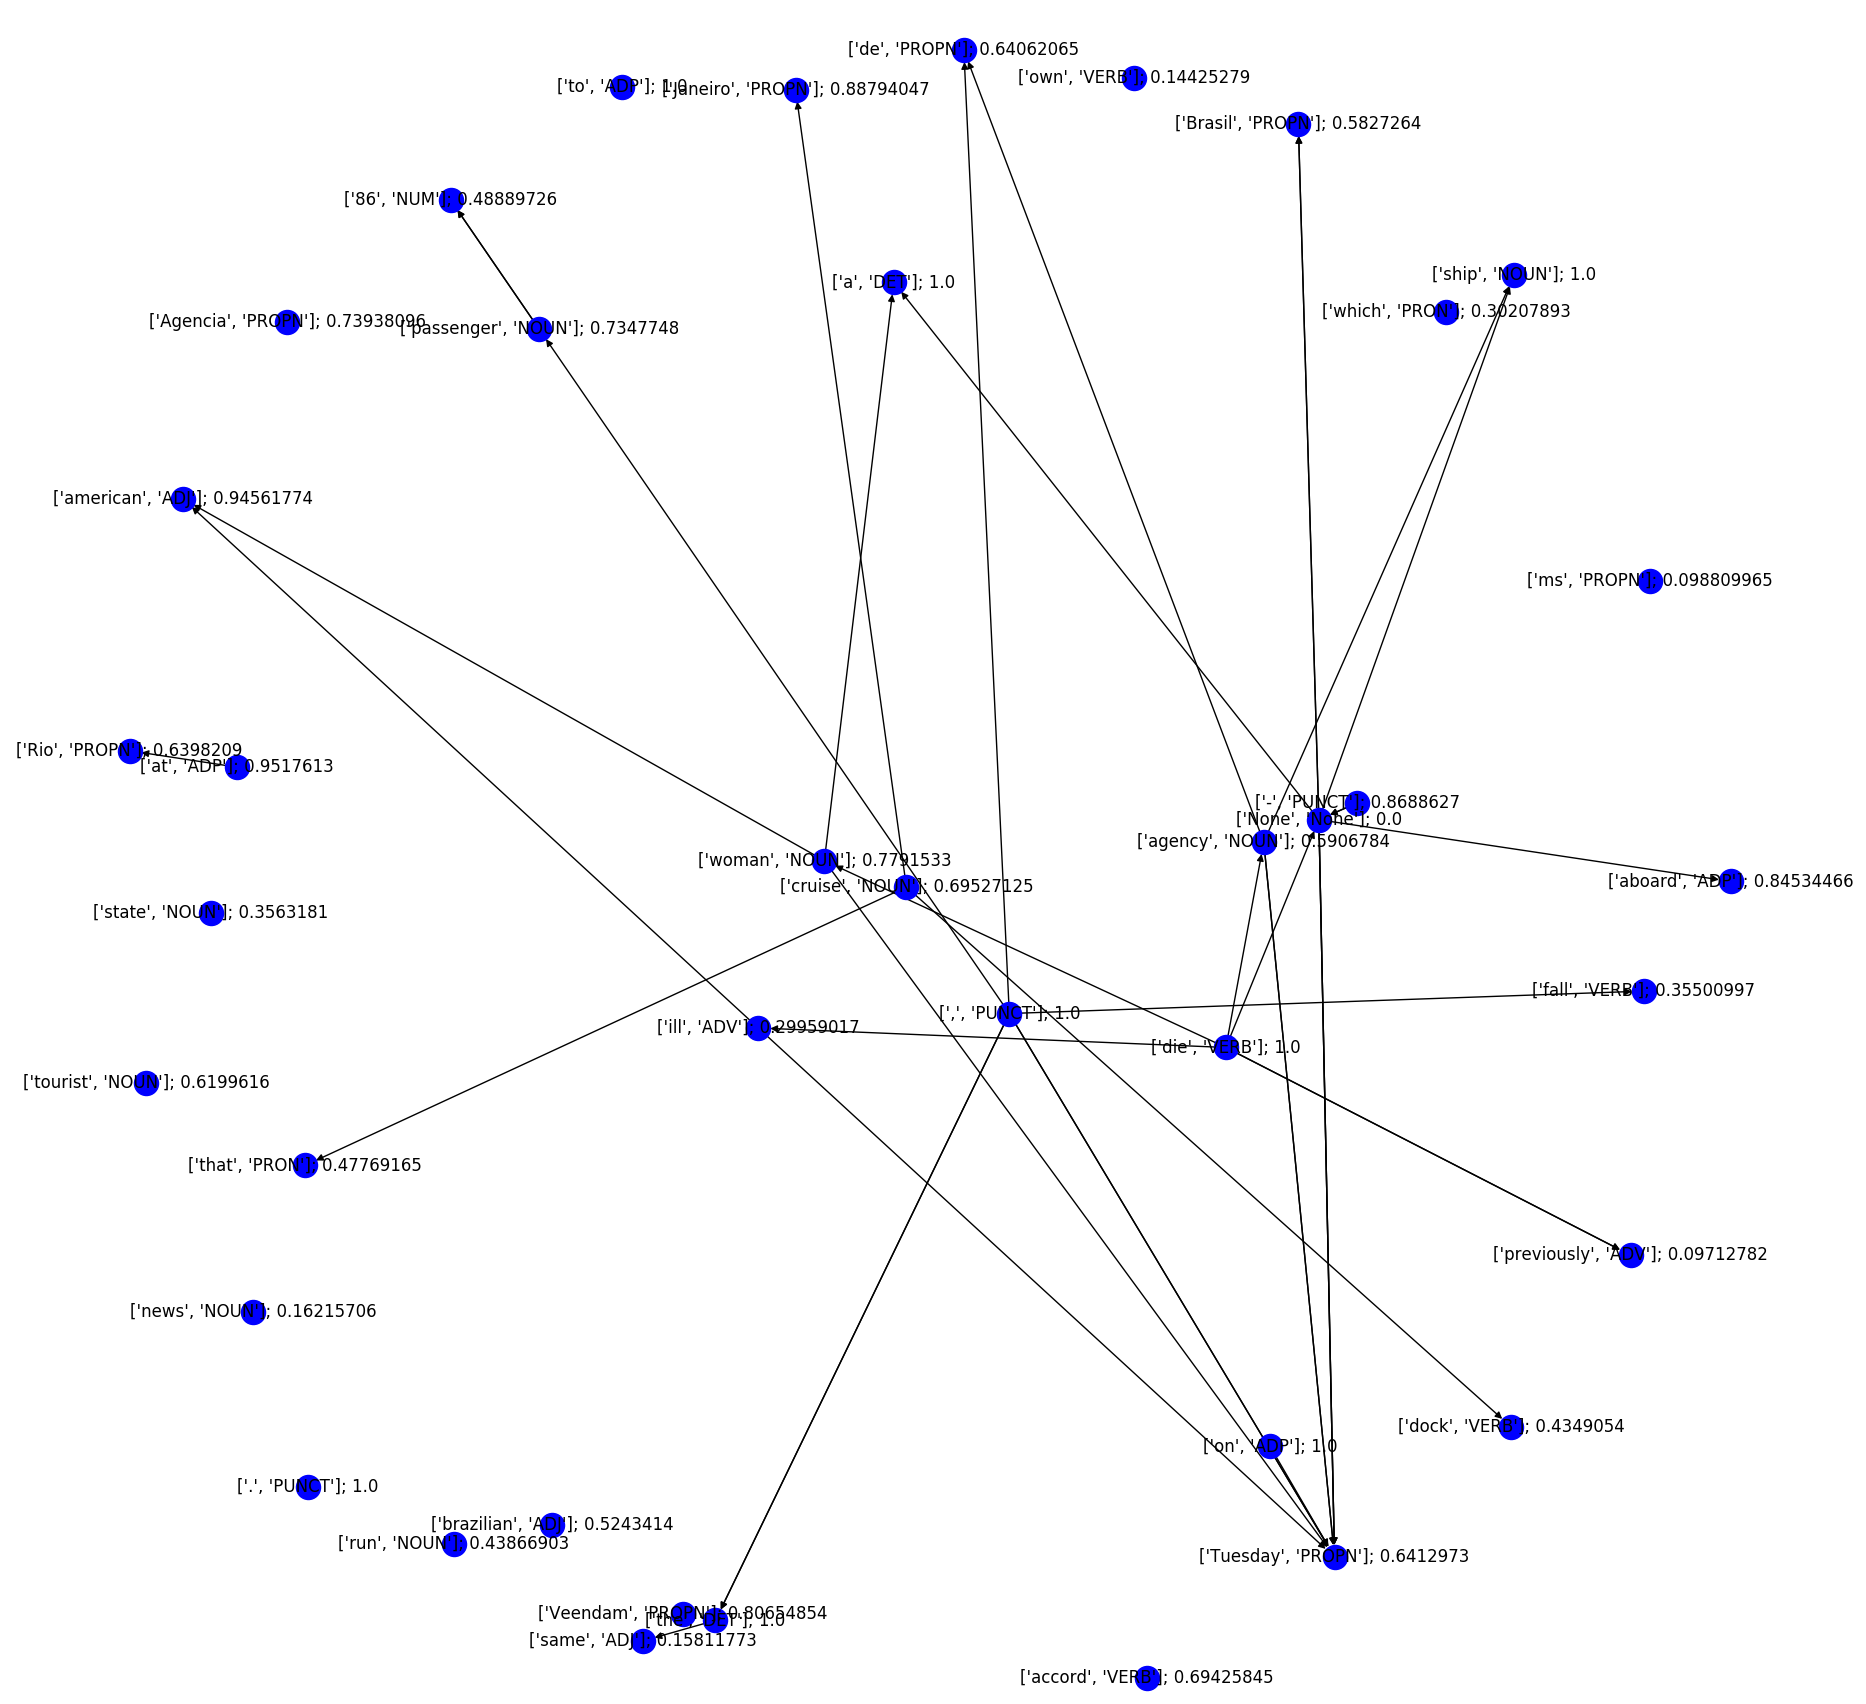
\includegraphics[width=150mm, keepaspectratio]{figures/small_predicted.png}
	\caption{The calculated summary graph of the short article with just the nodes labeled 1.}
	\label{fig:small_summary_calculated0}
\end{figure}

\textbox{
	\textbf{Reconstruction with the node average}
	
	The American tourist died aboard the MS Veendam, owned by cruise operator Holland America.
	An American woman died aboard a cruise ship that docked at Rio de Janeiro on Tuesday, the same ship on which 86 passengers previously fell ill, according to the state-run Brazilian news agency, Agencia Brasil.
	The ship's doctors told police that the woman was elderly and suffered from diabetes and hypertension, according the agency.
	The other passengers came down with diarrhea prior to her death during an earlier part of the trip, the ship's doctors said.
	
	\textbf{Reconstruction with just the graph structure}
	
	An American woman died aboard a cruise ship that docked at Rio de Janeiro on Tuesday, the same ship on which 86 passengers previously fell ill, according to the state-run Brazilian news agency, Agencia Brasil.
	The ship's doctors told police that the woman was elderly and suffered from diabetes and hypertension, according the agency.
	The other passengers came down with diarrhea prior to her death during an earlier part of the trip, the ship's doctors said.
	The American tourist died aboard the MS Veendam, owned by cruise operator Holland America.
	
	\textbf{Reconstruction with the graph structure and the node scores}
	
	An American woman died aboard a cruise ship that docked at Rio de Janeiro on Tuesday, the same ship on which 86 passengers previously fell ill, according to the state-run Brazilian news agency, Agencia Brasil.
	The American tourist died aboard the MS Veendam, owned by cruise operator Holland America.
	The ship's doctors told police that the woman was elderly and suffered from diabetes and hypertension, according the agency.
	The other passengers came down with diarrhea prior to her death during an earlier part of the trip, the ship's doctors said.}{
	\caption{Short article summaries}}

\begin{figure}[!ht]
	\centering
	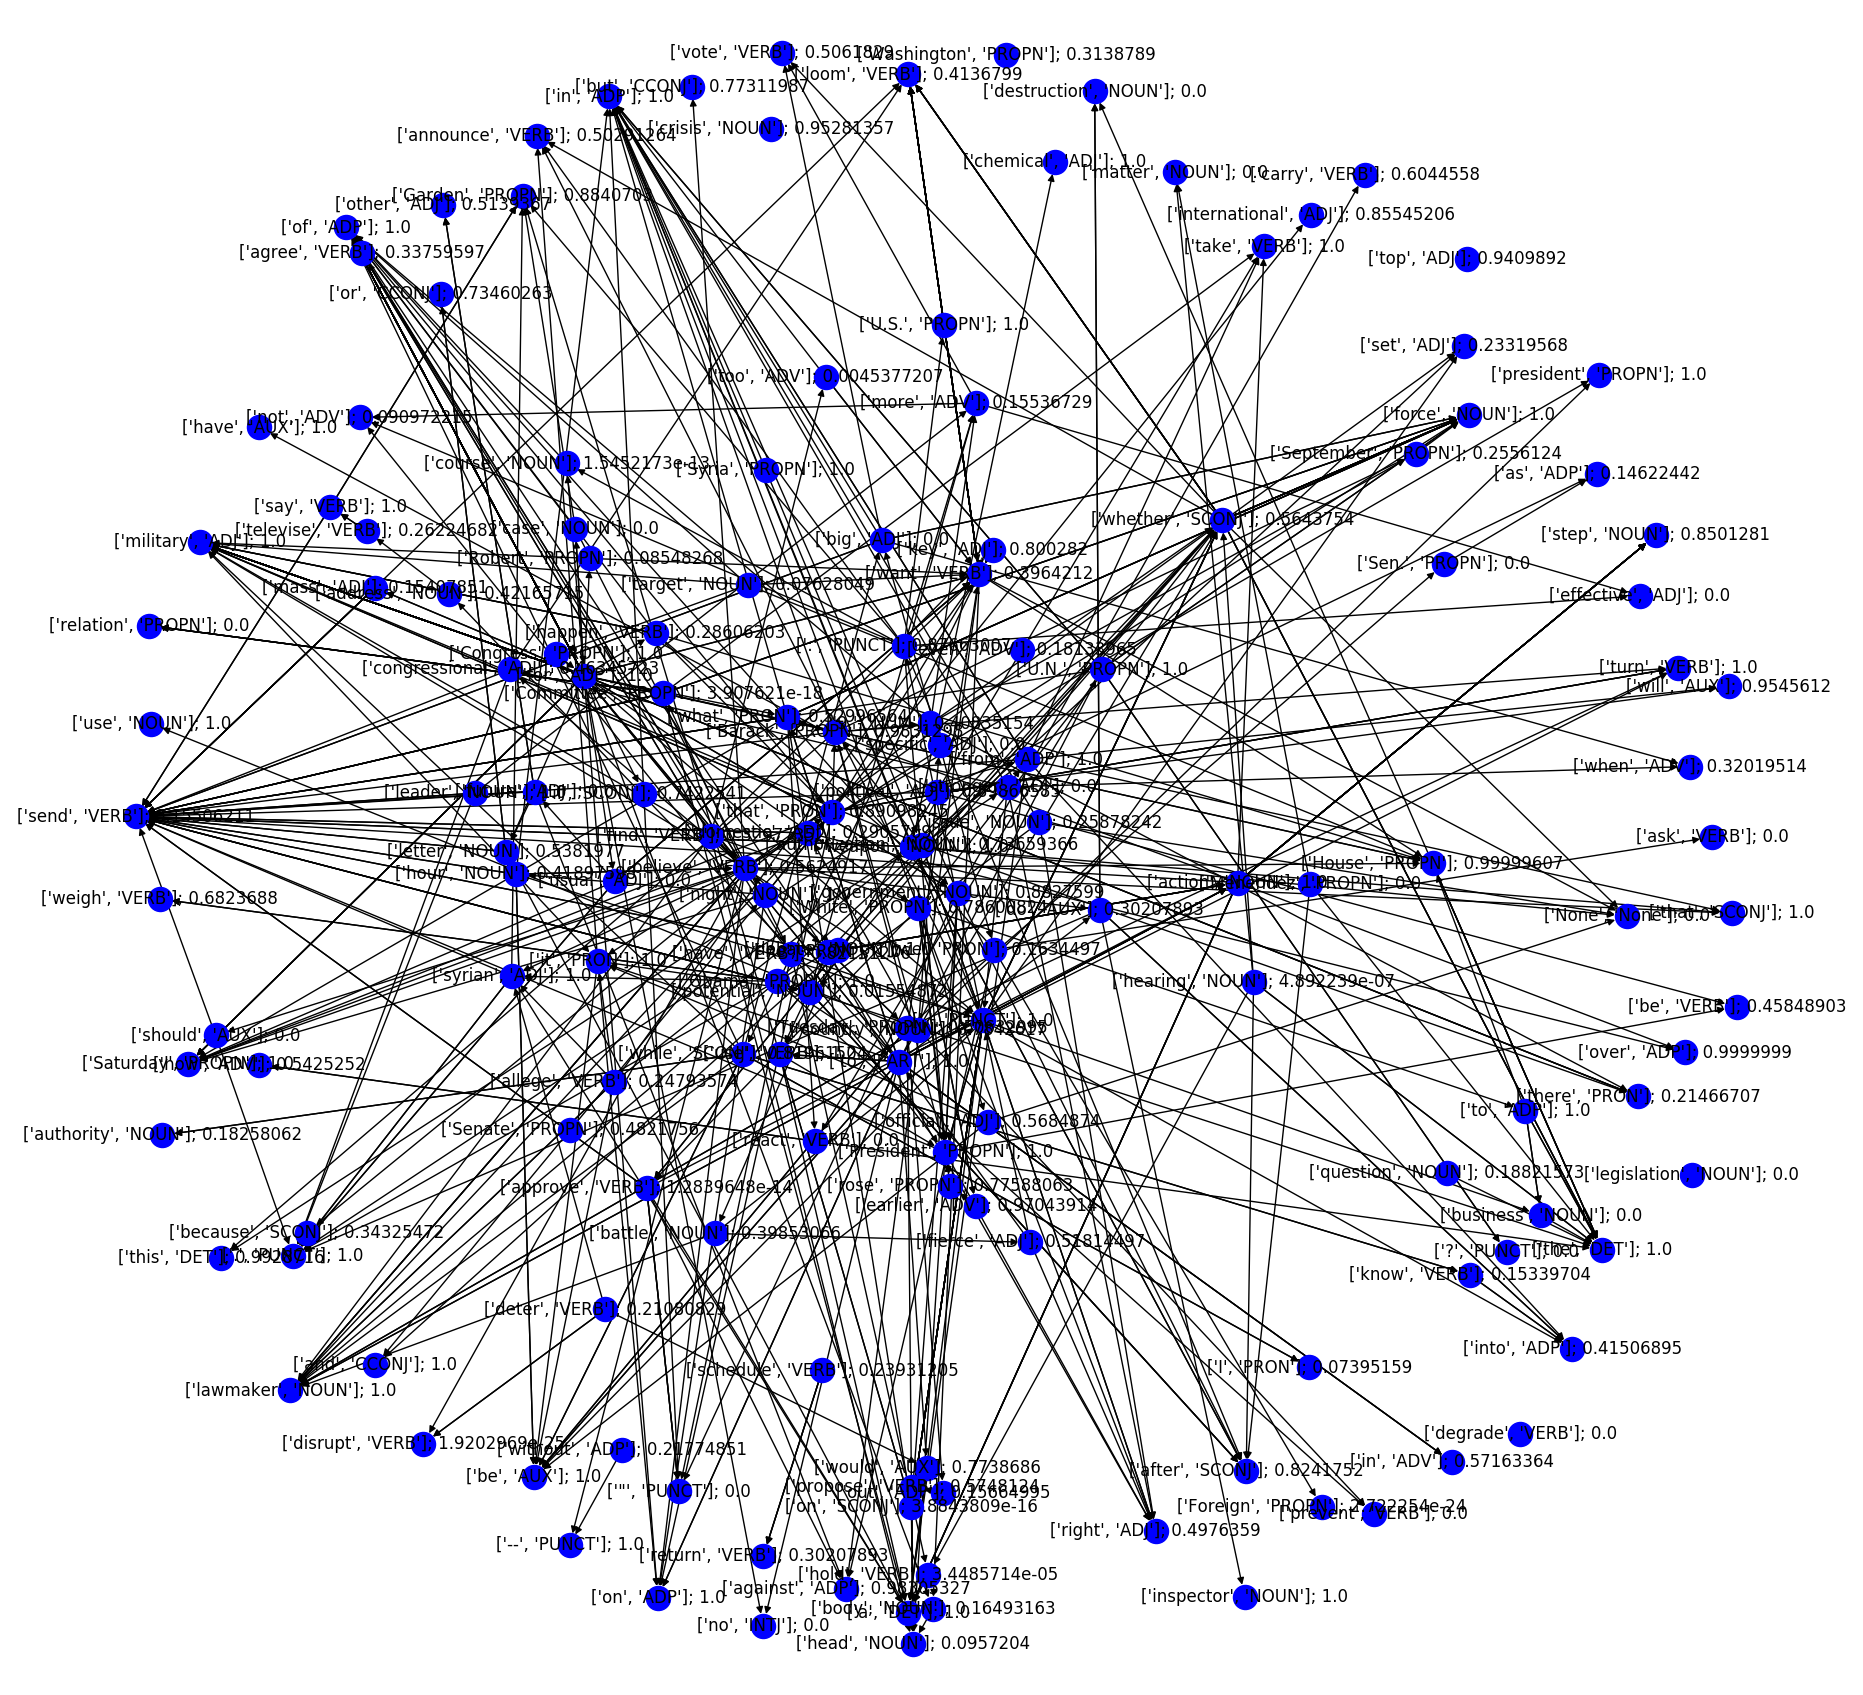
\includegraphics[width=150mm, keepaspectratio]{figures/large_predicted.png}
	\caption{The calculated summary graph of the normal length article with just the nodes labeled 1.}
	\label{fig:large_summary_calculated0}
\end{figure}

\textbox{
\textbf{Reconstruction with the node average}

It's official: U.S. President Barack Obama wants lawmakers to weigh in on whether to use military force in Syria.
There are key questions looming over the debate: What did U.N. weapons inspectors find in Syria?
U.N. inspectors leave Syria. 
Obama decision came Friday night.

\textbf{Reconstruction with just the graph structure}

"The Syrian Army's status is on maximum readiness and fingers are on the trigger to confront all challenges," Wael Nader al-Halqi said during a meeting with a delegation of Syrian expatriates from Italy, according to a banner on Syria State TV that was broadcast prior to Obama's address. "The main reason Obama is turning to the Congress:  the military operation did not get enough support either in the world, among allies of the US or in the United States itself," Alexei Pushkov, chairman of the international-affairs committee of the Russian State Duma, said in a Twitter post. "The two leaders agreed that the international community must deliver a resolute message to the Assad regime -- and others who would consider using chemical weapons -- that these crimes are unacceptable and those who violate this international norm will be held accountable by the world," the White House said. After Obama's speech, a military and political analyst on Syrian state TV said Obama is "embarrassed" that Russia opposes military action against Syria, is "crying for help" for someone to come to his rescue and is facing two defeats -- on the political and military levels.

\textbf{Reconstruction with the graph structure and the node scores}

Obama's remarks came shortly after U.N. inspectors left Syria, carrying evidence that will determine whether chemical weapons were used in an attack early last week in a Damascus suburb. The Syrian government has denied that it used chemical weapons in the August 21 attack, saying that jihadists fighting with the rebels used them in an effort to turn global sentiments against it. After Obama's speech, a military and political analyst on Syrian state TV said Obama is "embarrassed" that Russia opposes military action against Syria, is "crying for help" for someone to come to his rescue and is facing two defeats -- on the political and military levels. Obama sent a letter to the heads of the House and Senate on Saturday night, hours after announcing that he believes military action against Syrian targets is the right step to take over the alleged use of chemical weapons.}{
\caption{Normal length article summaries}}

\subsection{GraphAttention Network}
